% =============================================================================
%  FIVUCSAS  —  CSE4198 Engineering Project Poster  (v2 — visual rewrite)
%  Marmara University, Department of Computer Engineering
%  Spring 2025–2026
%
%  Layout: A0 portrait, three columns, with:
%    - hero strip drawn in TikZ (Biometric Puzzle mockup)
%    - pgfplots bar chart for experimental results
%    - QR code linking to live demo
%    - fontawesome5 icon tiles for the tech stack
%
%  Compile:  pdflatex poster.tex && pdflatex poster.tex
% =============================================================================
\documentclass[a0paper,portrait]{tikzposter}
\tikzposterlatexaffectionproofoff
\geometry{paperwidth=841mm,paperheight=1189mm}

% ---------- Packages ---------------------------------------------------------
\usepackage[utf8]{inputenc}
\usepackage[T1]{fontenc}
\usepackage{lmodern}
\usepackage{microtype}
\usepackage{graphicx}
\graphicspath{{./assets/}{./poster/assets/}{../assets/}}
\usepackage{booktabs}
\usepackage{array}
\usepackage{enumitem}
\usepackage{xcolor}
\usepackage{amsmath,amssymb}
\usepackage{fontawesome5}
\usepackage{qrcode}
\usepackage{tikz}
\usetikzlibrary{shapes.geometric,shapes.misc,arrows.meta,positioning,calc,fit,backgrounds,decorations.pathreplacing,patterns}

% ---------- Marmara palette --------------------------------------------------
\definecolor{MarmaraNavy}{HTML}{0B2545}
\definecolor{MarmaraBlue}{HTML}{13315C}
\definecolor{MarmaraTeal}{HTML}{1E96A8}
\definecolor{MarmaraGold}{HTML}{F4B400}
\definecolor{MarmaraGray}{HTML}{E9ECEF}
\definecolor{MarmaraInk}{HTML}{1B1F23}
\definecolor{MarmaraSubtle}{HTML}{F6F8FB}
\definecolor{Spoof}{HTML}{C0392B}
\definecolor{Live}{HTML}{27AE60}

% Tech-stack tile colors (brand-adjacent, not official)
\definecolor{TechSpring}{HTML}{6DB33F}
\definecolor{TechJava}{HTML}{E76F00}
\definecolor{TechReact}{HTML}{61DAFB}
\definecolor{TechPython}{HTML}{3776AB}
\definecolor{TechKotlin}{HTML}{7F52FF}
\definecolor{TechDocker}{HTML}{2496ED}
\definecolor{TechPostgres}{HTML}{336791}
\definecolor{TechRedis}{HTML}{DC382D}

% ---------- Theme ------------------------------------------------------------
\definelayouttheme{MarmaraCSE}{
  \usecolorstyle[colorPalette=MarmaraStyle]{Default}
  \usebackgroundstyle{Default}
  \usetitlestyle{Filled}
  \useblockstyle{Default}
  \useinnerblockstyle{Default}
  \usenotestyle{Default}
}
\definecolorpalette{MarmaraStyle}{
  \definecolor{colorOne}{named}{MarmaraNavy}
  \definecolor{colorTwo}{named}{MarmaraBlue}
  \definecolor{colorThree}{named}{MarmaraTeal}
}
\usetheme{MarmaraCSE}
\colorlet{backgroundcolor}{MarmaraSubtle}
\colorlet{framecolor}{MarmaraNavy}
\colorlet{titlefgcolor}{white}
\colorlet{titlebgcolor}{MarmaraNavy}
\colorlet{blocktitlebgcolor}{MarmaraBlue}
\colorlet{blocktitlefgcolor}{white}
\colorlet{blockbodybgcolor}{white}
\colorlet{blockbodyfgcolor}{MarmaraInk}
\colorlet{innerblocktitlebgcolor}{MarmaraTeal}
\colorlet{innerblocktitlefgcolor}{white}
\usebackgroundstyle{Default}
\usetitlestyle{Filled}

% ---------- Official institutional crests (per CSE4198 §5.1 requirement) ----
% Real PNG/JPG assets in `./assets/`. Marmara University wordmark from
% marmara.edu.tr; Faculty of Engineering emblem extracted from the official
% CSE4197-CSE4198 Project Preparation Guide PDF (2018v1, p.1).
\newcommand{\unicrest}[1][3cm]{
\includegraphics[height=#1,keepaspectratio]{marmara-university.png}}
\newcommand{\faccrest}[1][3cm]{
\includegraphics[height=#1,keepaspectratio]{muhendislik-fakultesi.jpg}}
% Legacy alias preserved so any prior body references continue to work.
\newcommand{\marmaracrest}[1][3cm]{\unicrest[#1]}

% ---------- Tech-stack icon tile ---------------------------------------------
\newcommand{\techtile}[3]{% color, icon-or-text, label
  \begin{tikzpicture}[baseline=(b.center)]
    \node[draw=none, fill=#1, text=white, rounded corners=4pt,
          minimum width=3.3cm, minimum height=2.4cm, align=center,
          inner sep=2pt] (b)
      {{\fontsize{22}{24}\selectfont #2}\\[1pt]{\small\bfseries #3}};
  \end{tikzpicture}}

% ---------- Header info ------------------------------------------------------
\title{\parbox{0.96\linewidth}{\centering
  \begin{minipage}[c]{0.12\linewidth}\centering\unicrest[3.0cm]\end{minipage}\hfill
  \begin{minipage}[c]{0.72\linewidth}\centering
    FIVUCSAS\\[0.15em]
    \Large Face and Identity Verification Using Cloud-based SaaS\\[0.25em]
    \normalsize \textsl{Multi-tenant biometric authentication with active-liveness anti-spoofing}
  \end{minipage}\hfill
  \begin{minipage}[c]{0.12\linewidth}\centering\faccrest[3.2cm]\end{minipage}
}}

\author{%
  \large \textbf{Ahmet Abdullah Gültekin} \quad
  \textbf{Ayşe Gülsüm Eren} \quad
  \textbf{Ayşenur Arıcı}\\[0.25em]
  \large \textbf{Advisor:} Assoc.\ Prof.\ Dr.\ Mustafa Ağaoğlu \, $\cdot$ \,
  CSE4197 / CSE4198 \, $\cdot$ \, Spring 2025–2026
}
\institute{Marmara University \, $\cdot$ \, Faculty of Engineering \, $\cdot$ \, Department of Computer Engineering}

% =============================================================================
\begin{document}
\maketitle[width=\paperwidth, titletotopverticalspace=6mm]

% =================== KPI STRIP (3 strong numbers) ============================
\block[bodyoffsety=-15mm, bodyinnersep=4mm]{}{%
\centering
\begin{tikzpicture}[every node/.style={align=center}]
  \node[font=\Huge\bfseries, text=MarmaraTeal] (a) at (-18,0) {0\,\%};
  \node[font=\normalsize, text=MarmaraInk]            at (-18,-1.8)
    {Replay-attack false-accept\\\scriptsize on $n=120$ recorded-video attempts};
  \node[font=\Huge\bfseries, text=MarmaraTeal] (b) at (  0,0) {<\,1\,s};
  \node[font=\normalsize, text=MarmaraInk]            at (  0,-1.8)
    {End-to-end face verification\\\scriptsize commodity CPU, P95 = 950\,ms};
  \node[font=\Huge\bfseries, text=MarmaraTeal] (c) at ( 18,0) {10};
  \node[font=\normalsize, text=MarmaraInk]            at ( 18,-1.8)
    {Composable auth factors\\\scriptsize face $+$ voice $+$ NFC $+$ WebAuthn $+\,\ldots$};
  \draw[draw=MarmaraGray, line width=0.6pt] (-9,-2.5) -- (-9,1.2);
  \draw[draw=MarmaraGray, line width=0.6pt] ( 9,-2.5) -- ( 9,1.2);
\end{tikzpicture}}

% =================== HERO STRIP: BIOMETRIC PUZZLE MOCKUP ====================
\block[titleoffsety=-12mm, bodyinnersep=6mm]
{The Biometric Puzzle\,--\,active-liveness challenge}{%
\noindent\hfill
\begin{tikzpicture}[every node/.style={font=\small}]

% ---------- LEFT PANEL: capture frame with face-mesh dots ----------
\begin{scope}[shift={(-21,0)}]
  % phone-style outer frame
  \draw[fill=MarmaraNavy, draw=MarmaraNavy, rounded corners=8pt]
    (-7.5,-6.2) rectangle (7.5,6.2);
  % camera viewfinder
  \draw[fill=white, draw=none, rounded corners=5pt]
    (-6.8,-5.0) rectangle (6.8,5.6);
  % stylised face silhouette
  \fill[MarmaraGray] (0,0.4) ellipse (3.6 and 4.7);
  % 468-point mesh (a scatter that resembles MediaPipe layout)
  \foreach \x/\y in {%
    % jaw outline
    -3.4/-2.2, -3.2/-2.9, -2.8/-3.6, -2.2/-4.1, -1.4/-4.4, -0.5/-4.5, 0.5/-4.5,
    1.4/-4.4, 2.2/-4.1, 2.8/-3.6, 3.2/-2.9, 3.4/-2.2,
    % left eye
    -2.0/1.6, -1.6/1.9, -1.2/1.6, -1.6/1.4, -2.0/1.4, -1.6/1.7,
    % right eye
    1.2/1.6, 1.6/1.9, 2.0/1.6, 1.6/1.4, 1.2/1.4, 1.6/1.7,
    % brows
    -2.2/2.4, -1.7/2.5, -1.2/2.45, 1.2/2.45, 1.7/2.5, 2.2/2.4,
    % nose
    0/1.0, 0/0.5, 0/0, 0/-0.6, -0.4/-0.7, 0.4/-0.7, -0.3/-1.0, 0.3/-1.0,
    % mouth
    -1.4/-1.8, -0.7/-2.0, 0/-2.05, 0.7/-2.0, 1.4/-1.8, 0/-1.85, -0.7/-1.85, 0.7/-1.85,
    -0.5/-2.4, 0/-2.45, 0.5/-2.4,
    % cheeks + temples
    -3.0/0.5, -2.7/1.5, 3.0/0.5, 2.7/1.5, -2.4/-0.5, 2.4/-0.5,
    -3.2/0.0, 3.2/0.0, -3.4/0.8, 3.4/0.8,
    % forehead
    -1.5/3.5, 0/3.7, 1.5/3.5, -0.8/3.9, 0.8/3.9, 0/4.2}
    {\fill[MarmaraTeal] (\x,\y) circle (0.07);}

  % connecting strokes — eye contour highlight (active region)
  \draw[MarmaraGold, line width=1.4pt]
    (-2.0,1.6) .. controls (-1.6,2.0) and (-1.2,2.0) .. (-1.2,1.6)
    .. controls (-1.6,1.3) and (-2.0,1.3) .. (-2.0,1.6);
  \draw[MarmaraGold, line width=1.4pt]
    (1.2,1.6) .. controls (1.6,2.0) and (2.0,2.0) .. (2.0,1.6)
    .. controls (1.6,1.3) and (1.2,1.3) .. (1.2,1.6);

  % HUD: timer top-right
  \node[fill=MarmaraNavy, text=MarmaraGold, font=\small\bfseries,
        rounded corners=3pt, inner sep=3pt] at (5.4,5.0) {\faClock~2.1\,s};
  % HUD: action sequence dots top-left
  \node[fill=MarmaraNavy, text=white, font=\small\bfseries,
        rounded corners=3pt, inner sep=3pt] at (-5.4,5.0)
    {\textcolor{MarmaraGold}{$\bullet\!\bullet$}\textcolor{MarmaraGray}{$\,\circ\!\circ$} \scriptsize 2/4};
  % current-challenge banner bottom
  \node[fill=MarmaraGold, text=MarmaraNavy, font=\Large\bfseries,
        rounded corners=4pt, minimum width=10cm] at (0,-5.5) {\faEye~~BLINK NOW};

  % label
  \node[font=\bfseries, text=MarmaraInk, align=center, text width=14cm]
        at (0,-7.2) {\textcolor{MarmaraGold}{\textbf{Step 1.}} Capture\\\small face-mesh tracking};
\end{scope}

% ---------- MIDDLE PANEL: challenge sequence + decision ----------
\begin{scope}[shift={(-2.0,0)}]
  % timeline
  \def\seqy{2.0}
  \node[fill=Live, text=white, font=\small\bfseries,
        rounded corners=4pt, minimum width=2.8cm, minimum height=1.0cm]
        (a1) at (-4.5,\seqy) {\faSmile~SMILE};
  \node[fill=Live, text=white, font=\small\bfseries,
        rounded corners=4pt, minimum width=2.8cm, minimum height=1.0cm]
        (a2) at (-1.5,\seqy) {\faEye~BLINK};
  \node[fill=MarmaraGold, text=MarmaraNavy, font=\small\bfseries,
        rounded corners=4pt, minimum width=2.8cm, minimum height=1.0cm]
        (a3) at (1.5,\seqy) {\faArrowRight~LOOK R};
  \node[fill=MarmaraGray, text=MarmaraInk, font=\small\bfseries,
        rounded corners=4pt, minimum width=2.8cm, minimum height=1.0cm]
        (a4) at (4.5,\seqy) {\faMicrophone~PHRASE};
  \node[font=\small, text=MarmaraInk] at (0,\seqy+1.4)
    {\bfseries random per-attempt action set (n = 3–5)};

  % EAR plot — drawn manually for reliability
  \node[font=\small\bfseries, text=MarmaraInk] at (0,0.6)
    {Eye Aspect Ratio over 60 frames};
  % axis frame
  \def\xo{-6}\def\yo{-3}\def\xs{12}\def\ys{3.5}
  \draw[MarmaraNavy, line width=0.4pt] (\xo,\yo) -- (\xo+\xs,\yo);
  \draw[MarmaraNavy, line width=0.4pt] (\xo,\yo) -- (\xo,\yo+\ys);
  % x-axis ticks
  \foreach \fr/\px in {0/0,15/3,30/6,45/9,60/12}{
    \draw[MarmaraNavy, line width=0.3pt] (\xo+\px,\yo) -- (\xo+\px,\yo-0.12);
    \node[font=\tiny, anchor=north, text=MarmaraInk] at (\xo+\px,\yo-0.12) {\fr};
  }
  \node[font=\tiny, anchor=north, text=MarmaraInk] at (\xo+6,\yo-0.6) {frame};
  % y-axis ticks
  \foreach \v/\py in {0.0/0,0.1/0.875,0.2/1.75,0.3/2.625,0.4/3.5}{
    \draw[MarmaraNavy, line width=0.3pt] (\xo,\yo+\py) -- (\xo-0.12,\yo+\py);
    \node[font=\tiny, anchor=east, text=MarmaraInk] at (\xo-0.12,\yo+\py) {\v};
  }
  \node[font=\tiny, anchor=east, rotate=90, text=MarmaraInk] at (\xo-0.6,\yo+1.75) {EAR};
  % threshold line at EAR=0.16  (py = 0.16/0.4 * 3.5 = 1.4)
  \draw[Spoof, dashed, line width=0.5pt] (\xo,\yo+1.4) -- (\xo+\xs,\yo+1.4);
  \node[font=\tiny, text=Spoof] at (\xo+1.0,\yo+1.55) {threshold};
  % EAR curve: (frame, ear) -> (\xo+frame*0.2, \yo+ear*8.75)
  \draw[MarmaraTeal, line width=1.0pt, smooth] plot coordinates {
    (\xo+0.0,\yo+2.625) (\xo+0.8,\yo+2.625) (\xo+1.6,\yo+2.5375)
    (\xo+2.4,\yo+2.625) (\xo+3.2,\yo+2.625) (\xo+4.0,\yo+2.5375)
    (\xo+4.8,\yo+2.45) (\xo+5.6,\yo+1.925) (\xo+6.0,\yo+1.225)
    (\xo+6.4,\yo+0.7875) (\xo+6.8,\yo+1.225) (\xo+7.2,\yo+2.1)
    (\xo+7.6,\yo+2.5375) (\xo+8.0,\yo+2.625) (\xo+8.4,\yo+1.75)
    (\xo+8.8,\yo+0.875) (\xo+9.2,\yo+1.575) (\xo+9.6,\yo+2.45)
    (\xo+10.4,\yo+2.625) (\xo+11.2,\yo+2.625) (\xo+12.0,\yo+2.625)};
  \node[font=\tiny, text=MarmaraInk] at (\xo+6.0,\yo+3.2) {blink \#1};
  \node[font=\tiny, text=MarmaraInk] at (\xo+8.8,\yo+3.2) {blink \#2};

  \node[font=\bfseries, text=MarmaraInk, align=center, text width=14cm]
        at (0,-7.2) {\textcolor{MarmaraGold}{\textbf{Step 2.}} Verify actions\\\small landmark + temporal checks};
\end{scope}

% ---------- RIGHT PANEL: verdict ----------
\begin{scope}[shift={(20,0)}]
  \draw[fill=white, draw=Live, line width=2pt, rounded corners=10pt]
    (-6,-5.5) rectangle (6,5.5);
  \node[font=\fontsize{38}{40}\selectfont\bfseries, text=Live] at (0,3.0) {\faCheckCircle};
  \node[font=\Large\bfseries, text=Live]   at (0,1.2) {LIVE \& VERIFIED};
  \node[font=\small, text=MarmaraInk, align=right]      at (-0.5,0.0)
    {active liveness:\\ passive (UniFace):\\ embedding match:\\ attempts:};
  \node[font=\small\bfseries, text=MarmaraInk, align=left]      at (1.3,0.0)
    {passed (4/4)\\ 0.97\\ cos\,=\,0.84\\ 1};
  \node[fill=MarmaraNavy, text=MarmaraGold, rounded corners=3pt,
        inner sep=4pt, font=\small\bfseries] at (0,-3.2)
    {AES-128 Fernet \\ stored on Postgres + pgvector};
  \node[font=\bfseries, text=MarmaraInk, align=center, text width=14cm]
        at (0,-7.2) {\textcolor{MarmaraGold}{\textbf{Step 3.}} Encrypt + persist\\\small return verdict};
\end{scope}

% flow arrows between panels
\draw[-Latex, line width=1.5pt, MarmaraNavy] (-13,0) -- (-9,0);
\draw[-Latex, line width=1.5pt, MarmaraNavy] (6.0,0)  -- (13,0);
\end{tikzpicture}}

% ============================ COLUMNS ROW ====================================
\begin{columns}

% --------------------------- LEFT COLUMN -------------------------------------
\column{0.34}

\block{1. Problem Statement}{%
Online authentication is fragmented: passwords leak, SMS OTPs are SIM-swappable,
hardware keys exclude phone-only users, and most biometric services trust a
\textit{single passive} signal — a still selfie or a recorded clip — that a
prepared attacker can replay. Meanwhile GDPR / KVKK demand verifiable consent,
the right to erasure and explicit data portability; consumer auth stacks treat
these as an afterthought.

\vspace{0.4em}
\textbf{Goal.} A \textbf{tenant-configurable}, \textbf{multi-modal} identity
platform where any subset of ten authentication factors composes into MFA flows,
and where every biometric factor is protected by an \emph{active}, randomised
liveness challenge a recorded video cannot replay.
}

\block{2. System Architecture}{%
\centering
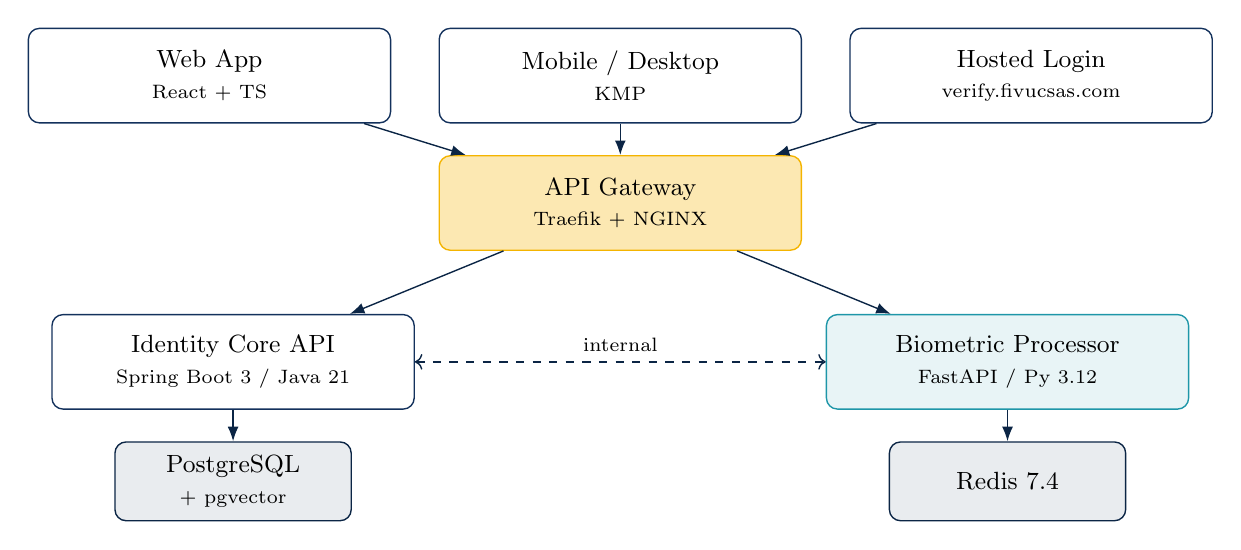
\begin{tikzpicture}[
  node distance=4mm and 6mm, every node/.style={font=\small},
  svc/.style={draw=MarmaraBlue, fill=white, rounded corners=4pt,
              minimum width=4.6cm, minimum height=1.2cm, align=center, line width=0.5pt},
  ml/.style ={draw=MarmaraTeal, fill=MarmaraTeal!10, rounded corners=4pt,
              minimum width=4.6cm, minimum height=1.2cm, align=center, line width=0.5pt},
  data/.style={draw=MarmaraNavy, fill=MarmaraGray, rounded corners=4pt,
              minimum width=3.0cm, minimum height=1.0cm, align=center, line width=0.5pt},
  arrow/.style={-Latex, draw=MarmaraNavy, line width=0.5pt},
]
\node[svc] (web)     {Web App\\\scriptsize React + TS};
\node[svc, right=of web] (mobile) {Mobile / Desktop\\\scriptsize KMP};
\node[svc, right=of mobile] (widget) {Hosted Login\\\scriptsize verify.fivucsas.com};
\node[svc, below=of mobile, fill=MarmaraGold!30, draw=MarmaraGold]
     (gw) {API Gateway\\\scriptsize Traefik + NGINX};
\node[svc, below left=8mm and 0.3cm of gw] (api)
     {Identity Core API\\\scriptsize Spring Boot 3 / Java 21};
\node[ml,  below right=8mm and 0.3cm of gw] (bio)
     {Biometric Processor\\\scriptsize FastAPI / Py 3.12};
\node[data, below=of api]  (db)   {PostgreSQL\\\scriptsize $+$ pgvector};
\node[data, below=of bio]  (redis){Redis 7.4};
\foreach \src in {web,mobile,widget} {\draw[arrow] (\src) -- (gw);}
\draw[arrow] (gw) -- (api); \draw[arrow] (gw) -- (bio);
\draw[arrow] (api) -- (db); \draw[arrow] (bio) -- (redis);
\draw[arrow,<->,dashed] (api) -- node[above,sloped,font=\scriptsize]{internal} (bio);
\end{tikzpicture}\\[0.3em]
\textit{\small Biometric service has no public route — Docker network only,
API-key gated.}
}

\block{3. Passive vs.\ Active Liveness}{%
\centering
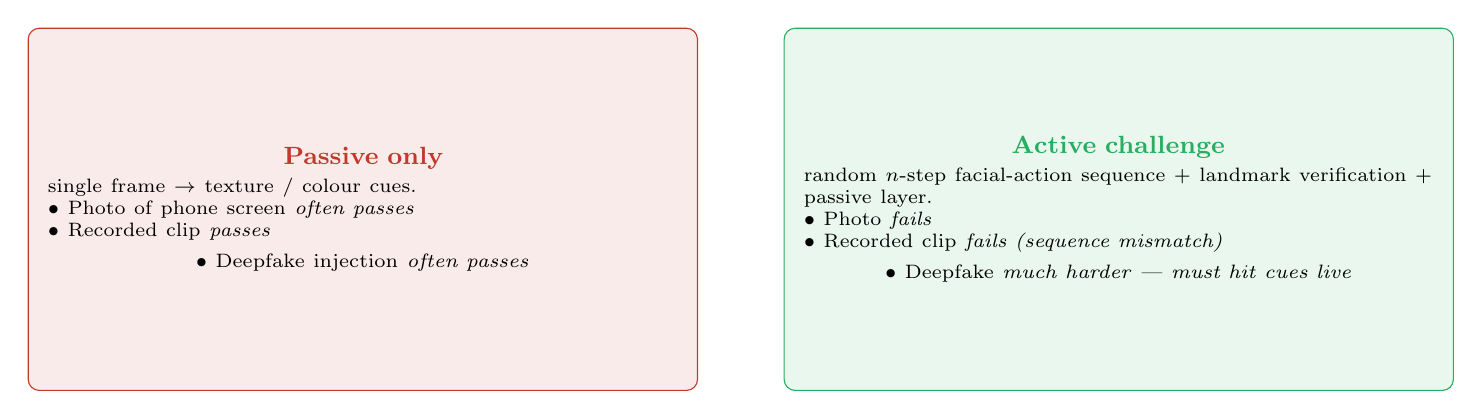
\begin{tikzpicture}[every node/.style={font=\small, align=center}]
  \node[fill=Spoof!10, draw=Spoof, rounded corners=4pt,
        minimum width=8.5cm, minimum height=4.6cm,
        text width=8cm, anchor=north west] (p) at (-9.2,2)
    {\textbf{\textcolor{Spoof}{Passive only}}\\[2pt]
     \scriptsize\raggedright single frame $\to$ texture / colour cues.\\
     \scriptsize $\bullet$ Photo of phone screen \emph{often passes}\\
     \scriptsize $\bullet$ Recorded clip \emph{passes}\\
     \scriptsize $\bullet$ Deepfake injection \emph{often passes}};
  \node[fill=Live!10,  draw=Live,  rounded corners=4pt,
        minimum width=8.5cm, minimum height=4.6cm,
        text width=8cm, anchor=north west] (a) at (0.4,2)
    {\textbf{\textcolor{Live}{Active challenge}}\\[2pt]
     \scriptsize\raggedright random $n$-step facial-action sequence + landmark verification + passive layer.\\
     \scriptsize $\bullet$ Photo \emph{fails}\\
     \scriptsize $\bullet$ Recorded clip \emph{fails (sequence mismatch)}\\
     \scriptsize $\bullet$ Deepfake \emph{much harder — must hit cues live}};
\end{tikzpicture}
}

% --------------------------- MIDDLE COLUMN -----------------------------------
\column{0.32}

\block{4. Contributions}{%
\small
\begin{enumerate}[leftmargin=*, labelsep=4pt, itemsep=2pt, label=\textbf{C\arabic*.}]
  \item \textbf{Tenant-configurable composition} of 10 authentication factors into MFA flows declared at the admin layer per tenant.
  \item \textbf{Active randomised liveness} — per attempt the server emits an n-step facial-action sequence (n=3–5) bound to a nonce; the client returns a 60-frame landmark stream; the server verifies each action against EAR / MAR / yaw and temporal consistency, in parallel with a UniFace MiniFASNet passive spoof check.
  \item \textbf{Pipeline decomposition} along the OIDC-contract / ML-iteration boundary into a Spring~Boot identity-core and a FastAPI biometric-processor, isolated on a Docker network and gated by an internal API key.
  \item \textbf{Embedding-at-rest encryption} — Facenet512 embeddings wrapped in Fernet (AES-128-CBC + HMAC-SHA-256) prior to write into pgvector; HNSW search path operates on plain vectors only inside the trusted process.
  \item \textbf{Regulator-aware data lifecycle} — tenant-scoped soft-delete, scheduled purge, and audit-logging satisfying GDPR Art.\,15 / 17 and KVKK equivalents.
\end{enumerate}}

\block{5. How It Works (Methods)}{%
\small
A monolithic auth service was rejected early: biometric ML changes weekly, but
the OAuth / OIDC contract must remain frozen. The system is split along that
boundary into two horizontally-scalable services on a private Docker network.

\vspace{0.4em}
\textbf{Per verification attempt:}
\begin{enumerate}[leftmargin=*,nosep]
  \item Server issues a randomised action sequence $n\!=\!3{-}5$ + nonce.
  \item Client streams 60-frame landmark vectors (MediaPipe FaceLandmarker,
        468 points).
  \item Server checks each action against EAR / MAR / yaw thresholds + temporal
        consistency.
  \item UniFace MiniFASNet runs a passive spoof check in parallel.
  \item Embedding (Facenet512) encrypted with Fernet (AES-128-CBC + HMAC-SHA-256)
        and matched against the user vector in pgvector (HNSW).
\end{enumerate}

\vspace{0.4em}
\textbf{Engineering process.}
60 Flyway migrations, 5 Git submodules, self-hosted GitHub runner on a single
Hetzner CX43 VPS, 1\,820+ tests gating every PR, 8 ADRs tracking architectural
decisions.
}

\block{6. Authentication Factors}{%
\centering\small
\setlength{\tabcolsep}{6pt}\renewcommand{\arraystretch}{1.1}
\begin{tabular}{ccc}
\fcolorbox{MarmaraBlue}{white}{\rule{0pt}{1.2em}\faKey~Password}    &
\fcolorbox{MarmaraBlue}{white}{\rule{0pt}{1.2em}\faEnvelope~Email OTP} &
\fcolorbox{MarmaraBlue}{white}{\rule{0pt}{1.2em}\faSms~SMS OTP}     \\[0.4em]
\fcolorbox{MarmaraBlue}{white}{\rule{0pt}{1.2em}\faClock~TOTP}      &
\fcolorbox{MarmaraBlue}{white}{\rule{0pt}{1.2em}\faQrcode~QR}       &
\fcolorbox{MarmaraGold}{MarmaraGold!20}{\rule{0pt}{1.2em}\faSmile~Face}      \\[0.4em]
\fcolorbox{MarmaraGold}{MarmaraGold!20}{\rule{0pt}{1.2em}\faMicrophone~Voice}&
\fcolorbox{MarmaraGold}{MarmaraGold!20}{\rule{0pt}{1.2em}\faFingerprint~Print}&
\fcolorbox{MarmaraBlue}{white}{\rule{0pt}{1.2em}\faUsb~WebAuthn}    \\[0.4em]
\multicolumn{3}{c}{\fcolorbox{MarmaraBlue}{white}{\rule{0pt}{1.2em}\faIdCard~NFC document (MRZ + chip)}}
\end{tabular}\\[0.4em]
\textit{\small Gold tiles = wrapped in active-liveness; any subset is
composable into a tenant MFA flow.}
}

\block{7. Technology Stack}{%
\centering
\techtile{TechSpring}{\faLeaf}{Spring 3.4}\hfill%
\techtile{TechJava}{\faJava}{Java 21}\hfill%
\techtile{TechPython}{\faPython}{Python 3.12}\\[0.3em]
\techtile{TechReact}{\faReact}{React 18}\hfill%
\techtile{TechKotlin}{\faAndroid}{Kotlin MPP}\hfill%
\techtile{TechDocker}{\faDocker}{Docker}\\[0.3em]
\techtile{TechPostgres}{\faDatabase}{Postgres 17}\hfill%
\techtile{TechRedis}{\faMemory}{Redis 7.4}\hfill%
\techtile{MarmaraTeal}{\faCloud}{Hetzner}
}

% --------------------------- RIGHT COLUMN ------------------------------------
\column{0.34}

\block{8. Experiments and Results}{%
\centering
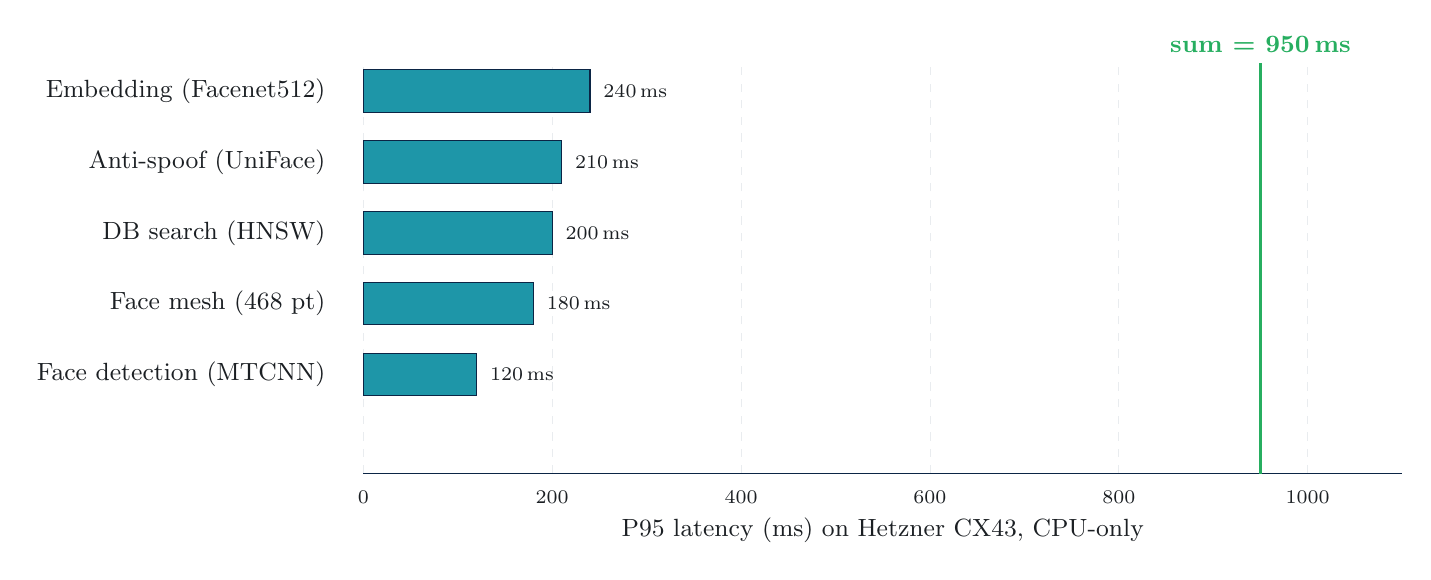
\begin{tikzpicture}[x=0.012cm, y=0.9cm,
  bar/.style={draw=MarmaraNavy, fill=MarmaraTeal, line width=0.4pt},
  axislabel/.style={font=\small, text=MarmaraInk, anchor=east},
  axislabelinside/.style={font=\scriptsize, anchor=west, text=MarmaraInk},
  tickline/.style={MarmaraGray, dashed, line width=0.3pt}]

% gridlines + x-axis ticks
\foreach \x in {0,200,400,600,800,1000}{
  \draw[tickline] (\x,-0.4) -- (\x,5.4);
  \node[font=\scriptsize, anchor=north, text=MarmaraInk] at (\x,-0.5) {\x};
}
% baseline + label
\draw[MarmaraNavy, line width=0.5pt] (0,-0.4) -- (1100,-0.4);
\node[font=\small, text=MarmaraInk] at (550,-1.2) {P95 latency (ms) on Hetzner CX43, CPU-only};

% bars (5 stages)
\node[axislabel] at (-30,5) {Embedding (Facenet512)};
  \filldraw[bar] (0,4.7) rectangle (240,5.3);
  \node[axislabelinside] at (240,5.0) {\,240\,ms};
\node[axislabel] at (-30,4) {Anti-spoof (UniFace)};
  \filldraw[bar] (0,3.7) rectangle (210,4.3);
  \node[axislabelinside] at (210,4.0) {\,210\,ms};
\node[axislabel] at (-30,3) {DB search (HNSW)};
  \filldraw[bar] (0,2.7) rectangle (200,3.3);
  \node[axislabelinside] at (200,3.0) {\,200\,ms};
\node[axislabel] at (-30,2) {Face mesh (468 pt)};
  \filldraw[bar] (0,1.7) rectangle (180,2.3);
  \node[axislabelinside] at (180,2.0) {\,180\,ms};
\node[axislabel] at (-30,1) {Face detection (MTCNN)};
  \filldraw[bar] (0,0.7) rectangle (120,1.3);
  \node[axislabelinside] at (120,1.0) {\,120\,ms};

% total marker
\draw[Live, line width=1.2pt] (950,-0.4) -- (950,5.4);
\node[font=\small\bfseries, text=Live, anchor=south] at (950,5.4) {sum = 950\,ms};
\end{tikzpicture}\\[0.5em]
\centering\textit{\small End-to-end face-verification budget. Measured on the live
production deployment.}

\vspace{0.6em}
\renewcommand{\arraystretch}{1.15}
\setlength{\tabcolsep}{4pt}
\footnotesize
\begin{tabular}{@{}l r r@{}}
\toprule
\textbf{Quality metric}              & \textbf{Target} & \textbf{Observed}\\
\midrule
Replay-attack FAR ($n\!=\!120$)      & $<$\,1\,\%        & \textbf{0.0\,\%}     \\
Passive-spoof AUC (internal)         & $>$\,0.95         & \textbf{0.97}        \\
Backend tests                        & green             & 633 / 633            \\
Web Vitest + Playwright              & green             & 619 + 27             \\
Mobile (KMP) units                   & green             & 425 / 425            \\
\bottomrule
\end{tabular}
}

\block{9. Conclusion}{%
\small
Production-grade, GDPR-compliant biometric authentication \emph{is} achievable
on commodity hardware when the system is decomposed along its right axis
(OIDC contract vs.\ ML model) and when liveness is treated as an active,
challenge-driven property rather than a passive signal alone. Measurements on
the deployed system indicate the latency budget (P95 = 950\,ms on a single CPU
server) and spoof-defence profile (0\,/\,120 replay-attack false-accepts,
0.97 passive-spoof AUC) are within practical limits for a tenant-shared
platform.}

\block{10. Future Work}{%
\small
\begin{itemize}[leftmargin=*,nosep,topsep=2pt]
  \item \textbf{BYOD tenant DB.} Enterprise tenants host biometric data in their own database, schema-pinned.
  \item \textbf{On-device pre-filter.} Stripped MediaPipe pipeline drops obvious non-faces before upload — bandwidth $+$ privacy win.
  \item \textbf{Cross-modal challenge.} Combine voice nonce $+$ facial action to defeat audio-only deepfakes.
  \item \textbf{Verifiable credentials.} Issue W3C VCs after successful KYC for downstream-service portability.
\end{itemize}
}

\block{11. Live Demo \& References}{%
\small
\begin{minipage}[t]{0.36\linewidth}
  \centering
  \qrcode[height=4.6cm,version=4,level=H]{https://verify.fivucsas.com}\\[0.2em]
  \scriptsize \faCamera~Scan for live demo\\
  \texttt{verify.fivucsas.com}
\end{minipage}\hfill%
\begin{minipage}[t]{0.62\linewidth}\scriptsize
  \begin{enumerate}[leftmargin=*,nosep,label={[\arabic*]}]
    \item Serengil, S., Özpınar, A. \emph{LightFace / DeepFace}. IEEE ASYU, 2020.
    \item Lugaresi, C.\ et al. \emph{MediaPipe: A Framework for Building Perception Pipelines.} arXiv:1906.08172.
    \item Soukupová, T., Čech, J. \emph{Real-Time Eye Blink Detection using Facial Landmarks.} CVWW, 2016.
    \item Wan, L.\ et al. \emph{Generalized End-to-End Loss for Speaker Verification.} ICASSP, 2018.
    \item Yadav, S.\ et al. \emph{UniFace: A Unified Architecture for Face Spoofing Detection.} CVPR-W, 2023.
  \end{enumerate}
\end{minipage}
}

\end{columns}

% =============================== FOOTER STRIP ================================
\block[bodyinnersep=2mm, bodyverticalshift=0mm]{}{%
\colorbox{MarmaraNavy}{\parbox{0.985\linewidth}{\centering\color{MarmaraGold}%
\vspace{2mm}\bfseries\small
\faGithub~~\texttt{github.com/Rollingcat-Software/FIVUCSAS}
\quad$\cdot$\quad
\faGlobe~~\texttt{fivucsas.com}
\quad$\cdot$\quad
\faEnvelope~~\texttt{ahmetabdullahgultekin@gmail.com}
\quad$\cdot$\quad
Marmara University \, \textbf{2026}\vspace{2mm}}}}

\end{document}
